\textit{	
	\begin{itemize}
		\item[-] General framework of multistratum experiments. [add more on model uncertainty]
		\item[-] Error estimation: REML and pure error REML. Yates procedure
		\item[-] Adapting optimality criteria and design construction
	\end{itemize}
}

In a large number of industrial, engineering and laboratory-based experiments, either the nature of the study or certain restrictions result in the necessity of considering a multi-level structure of experimental units. For example, a chemical process consisting of applying treatments to the material batches of different sizes at each stage;  or one or several experimental factors' values can be changed only once per a certain amount of runs whereas values of other factors are varied between runs. Therefore, different factors are applied at different levels, and randomisation is performed at each level, thus the whole process of allocating treatments to experimental units should be amended accordingly \citep{MeadGilmour2012}.

In this work we go on to consider experimental framework comprising such a hierarchical structure of experimental units and treatments, which is referred to as multistratum experiment, and each stratum is defined as a level in the unit structure. Units are grouped into whole-plots, each of them divided into sub-plots, which contain a certain number of sub-sub-plots, and so on up to the smallest units --- runs of the experiment -- [Figure .with Hasse diagram?] . In the general case of two strata, we deal with what is called a ``split-plot'' experiment, in case of three strata a ``split-split-plot'' experiment. 
%\begin{figure}[h]
%	\begin{center}
%		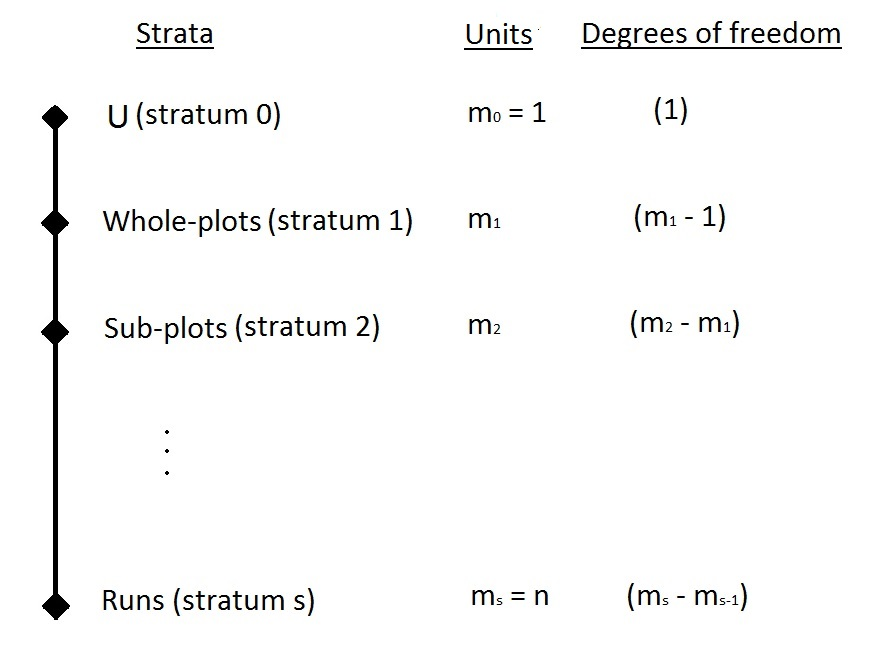
\includegraphics[scale=0.85]{Hasse.jpg}      %width=\textwidth
%		\caption{Hasse diagram for factors}
%		\label{Fig::Hasse}
%	\end{center}
%\end{figure} 
Our aim is to adapt the MSE-based criteria derived before to the factorial experiments with units distributed in several strata. The most important aspects are (1) estimating the error components at all of the levels and (2) formulating the compliant criteria and provide the suitable implementation strategy for the optimal design search.

\subsection{Response-Surface Methodology for multistratum framework}
%% Model. Ratio of variances.
[OE: introduce the notion of "block"?]
Here we are considering experiments with $s$ strata in total, stratum $i$ being nested within units of the stratum $i-1$, and stratum $0$ will be seen as the whole experiment (following the notation set by \citet{Trinca2015improved}). The number of units in stratum $i$ within every unit in stratum $i-1$ is denoted by $n_i$, such that $m_{j}=\prod_{i=1}^{j}n_{i}$ is the number of units in stratum $j$ and, therefore,  $n=m_{s}=\prod_{i=1}^{s}n_{i}$ is the total number of runs. As randomisation occurs at each stratum, the model accounting for the hierarchical error structure and correlated observations can be written as
\begin{equation}
\label{eq::MS_model}
\bm{Y}=\bm{X}\bm{\beta}+\sum_{i=1}^{s}\bm{Z}_{i}\bm{\varepsilon}_{i},
\end{equation}
where $\bm{Y}$ represents the $n$-dimensional vector of responses, $\bm{X}$ stands for the $n \times p$ model matrix and $\bm{\beta}$ for the $p$-dimensional vector of corresponding model coefficients. Each row of the $n\times m_{i}$ matrix $\bm{Z}_{i}$ corresponds to a single experimental run and indicates the unit in stratum $i$ containing this run. $\bm{\varepsilon}_{i}$ is a vector of random effects occurring due to the randomisation at level $i$, and these effects are assumed to be independent and identically distributed around zero mean and variance $\sigma^{2}_{i}$. Generalised Least Squared  (GLS) estimators of $\bm{\beta}$ are calculated as
\begin{equation}
\label{eq::MS_GLS}
\bm{\hat{\beta}}=(\bm{X}'\bm{V}^{-1}\bm{X})^{-1}\bm{X}'\bm{V}^{-1}\bm{Y}.
\end{equation}

%The assumption of error normality, though quite common is required for some analysis methods, is not a necessary one at this stage.

%Inferential purposes of obtaining parameter estimates $\bm{\hat{\beta}}$ of good quality imply the necessity of evaluating the dispersion parameters $\sigma^2_{i}$ that are directly related to the estimates' variance and, therefore, responsible for measuring the uncertainty of the inference in a general sense.

\subsubsection*{Error Estimate}
An extensive amount of research has been conducted on the design of and analysis of data from split-plot and split-split-plot experiments, with one of the first works by \cite{Letsinger1996BiRandomization}, emphasising the necessity of adapting the design and analysis strategy with respect to the more complicated error structure.  In the most general case of non-orthogonal unit structures Residual Maximum Likelihood (REML) methodology has been acknowledged to be the most sensible approach to estimating the variance components by maximising the part of the likelihood function corresponding to the ``random'' part of the model; the details are provided, for example, in \cite{Searle2001generalized}. 

%In traditional REML-based methodology the estimates of $\sigma^{2}_{i}$ are obtained from model (\ref{eq::MS_model}) and then GLS estimators of $\bm{\beta}$ are calculated as
%\begin{equation}
%\label{eq::MS_GLS}
%\bm{\hat{\beta}}=(\bm{X}'\bm{V}^{-1}\bm{X})^{-1}\bm{X}'\bm{V}^{-1}\bm{Y},
%\end{equation}
%where $\bm{V}$ is the unknown variance-covariance matrix of the response vector, to which the estimates are to be plugged in:
%\begin{equation*}
%\bm{V}=\sum_{i=1}^{s}\sigma^{2}_{i}\bm{Z}_{i}\bm{Z}'_{i},
%\end{equation*}
%so that $\mbox{Var}(\bm{\hat{\beta}})=(\bm{X}'\bm{V}^{-1}\bm{X})^{-1}.$

In some case, though,  REML tends to underestimate the variance components in the higher stratum, for example \cite{Goos2006practical} considered some split-plot experiments with true whole-plot variances being non-negligibly far from zero, for which REML, however, provided zero estimates. A possible alternative of following Bayesian strategy \citep{Gilmour2009analysis}, however, this requires a careful choice of the prior which is often not possible, especially in the case of more than two strata.

In the context of model uncertainty, it would be appropriate to consider instead the direct relationship between the response and the set of treatments, similar to (\ref{eq::treatment_model}):
\begin{equation}
\label{eq::treatmentMS}
\bm{Y}=\bm{X_t}\bm{\mu_t}+\sum_{i=1}^{s}\bm{Z}_{i}\bm{\varepsilon}_{i}.
\end{equation}

Each column of $\bm{X_t}$ corresponds to a treatment defined as a combination of the experimental factors;
%in case of factorial experiment the total number of possible treatments (or candidate design points) $T$ would be the product of the number of the factors' levels. 
$\bm{Z}_{i}$ is the indicator matrix of random effects at stratum $i$.

\cite{GilmourGoos2016PEREML} introduced the notion of ``Pure Error REML'', where random effects are estimated from the treatment model (\ref{eq::treatmentMS}), and then for the sake of making inference regarding parameters of the response model (\ref{eq::MS_model}), they are substituted in the GLS estimators of the fixed effects (\ref{eq::MS_GLS}). It is also argued that some appropriate corrections are to be adapted and applied to the obtained estimates, i.e.~the ones suggested by \cite{kenward1997small}. 

A careful definition of ``pure error'' is necessary when considering the treatment and response surface models, especially in the presence of nested random block effects. \cite{Gilmour2000PErsm} discuss the pure error estimation issues in the context of blocked experiments. 

[OE: The following is to be paraphrased -- made much shorter or removed overall?]
Pure error is expected to measure the variability between experimental units regardless of the treatments applied, and therefore, the assumption of treatment-unit additivity is essential in unblocked experiments.  In the presence of one or several blocking factors, the existence of block-treatment interaction would imply that pure error in the lower strata can only be estimated from the replicates within blocks, so that inter-block information is not taken into consideration. Hence, in the blocked cases the assumption of treatment-block additivity \citep{Draper1998} is desirable. \cite{Gilmour2000PErsm} argue for the preservation of treatment-unit additivity when either fixed or random block effects are in the model in order to preserve consistency with the unblocked experiments; that would also conveniently imply treatment-block additivity. Adoption of these assumptions would then lead to the following representation of the relationship between responses and treatments in multi-stratum experiments. 

The outcome of applying treatment $i$ $(i=1\ldots T)$ to the experimental run located in the units $j_1$ of the first stratum, $j_2$ of the second stratum, $\ldots$ , and unit $j_s$ of the $s-$th stratum can be expressed as follows:
\begin{equation}
\label{eq::ms_tr}
y_{ij_{1}...j_{s}}=\mu+t_{i}+b_{j_1}+\ldots +b_{j_s},
\end{equation}
where $b_{j_s}$ is usually denoted as between-run variation. 

Under the stronger assumption of the response surface model (\ref{eq::MS_model}), the treatment effects $t_{i}$ are represented as a set of polynomial model terms.  

Based on the interrelation of the two models, and the desirability of being able to provide the possibility for testing for the lack-of-fit together with obtaining robust estimates of the variance components, the approach of using pure error is adopted, \cite{GilmourGoos2016Robust} explored several approaches to estimating the variance components. \\[5 pt]
[OE: the end of the part to be re-written/excluded]

The first approach is stratum-by-stratum data analysis, where each randomisation level is considered separately, and at each stratum $i$ units are treated as runs aggregated in $m_{i-1}$ blocks with fixed effects. The lower stratum variance is estimated from within blocks (using intra-block residual mean square), and the higher stratum (inter-block) variance from the difference between the intra- and inter-block residual mean squares scaled by the number of runs per block \citep{Hinkelmann2005Advanced}. This strategy requires only the treatment-unit additivity assumption and provides unbiased treatment effects' estimators. However, it would be desirable to make use of combining information not just from within-strata (intra-block) treatment replicates, but also from between-strata (inter-block) ones, especially in the common cases of relatively small experiments when the amount of runs available does not allow for obtaining higher stratum variance components from only considering blocks as whole units. Yates' procedure, first suggested by \cite{yates1939recovery} and described in detail by \cite{Hinkelmann2005Advanced}, provides more degrees of freedom for the variance estimate in the higher stratum -- and this is the approach we are adopting in this work. 

In the case of two levels of randomisation, variance components are estimated in two variance decomposition steps: 
\begin{enumerate}
	\item Total SS = SS(Blocks) + SS(Treatments$\vert$Blocks) + SS(Residual)\\
	From fitting this full treatment-after-blocks model the residual mean square $S^2$ is taken as the estimate of the intra-block variance. SS(Residual) is then substituted in the following partition.
	\item Total SS = SS(Treatments) + SS(Blocks$\vert$Treatments) + SS(Residual)\\
	Therefore, the sums of squares for the blocks after the treatment effects have been accounted for is obtained and the corresponding mean square $$S^2_{b}=\mbox{SS(Blocks$\vert$Treatments)}/\nu_{b}$$ is then used to get an estimate of the inter-block variance:
	$\hat{\sigma}^2_{b}=\frac{\nu_{b}(S^2_{b}-S^2)}{d}$,
	where pure error degrees of freedom for inter-block variance is $d=n-\mbox{trace}[\bm{Z}'\bm{X_t}(\bm{X_t}'\bm{X_t})^{-1}\bm{X_t}'\bm{Z}]$, $\nu_{b}=\mbox{rank}([\bm{X_t} \bm{Z}])-\mbox{rank}(\bm{X_t})$, and $\bm{X_t}$ and $\bm{Z}$ are as in (\ref{eq::treatmentMS}).
\end{enumerate}

Allocation of the degrees of freedom in practice, following Yates' procedure, is provided in the Appendix. 

[OE: to shorten]\\
\cite{GilmourGoos2016Robust} show that in addition to the treatment-unit additivity and randomisation the assumption of the experimental units being a random sample from an infinite population is necessary for the inter-block variance estimate to be unbiased. In this particular context, when the normality and independence of responses in (\ref{eq::MS_model}) is a standard assumption, although a potential presence of contamination effects in the fixed part of the model is also accounted for, Yates' approach seems to be the most appropriate technique. However, relying on the distribution assumption to the extent that makes REML the most sensible approach means that the fixed part of the fitted model is assumed to be absolutely true, that is the parameters of the population distribution are known, which does not comply with the model uncertainty framework. 

Together with the specifications regarding estimation of the variance components, it is necessary to carefully establish the way the pure error degrees of freedom should be determined and how the available remaining number of treatment degrees of freedom would be distributed between the polynomial, lack-of-fit and inter-block information components. 

\subsection{MSE-based compound criteria for multistratum experiments}
\label{sec::ch7_search}
In the presence of potential model disturbance which is expressed as additional polynomial terms, the full model for a multistratum experiment is then:
\begin{equation}
\label{eq::MS_model_full}
\bm{Y}=\bm{X}_p\bm{\beta}_p+\bm{X}_q\bm{\beta}_q+\sum_{i=1}^{s}\bm{Z}_{i}\bm{\varepsilon}_{i},
\end{equation}
where $\bm{X}_p$ is the primary terms matrix, and $bm{X}_q$ contains potential terms.

The design construction will follow the approach developed by \cite{Trinca2015improved}: an iterative, stratum-by-stratum algorithm, that treats the higher stratum units as fixed blocks; such an approach does not require any prior assumptions regarding the values of the variance components. 

At each step a candidate set of treatments applied at the current stratum is to be generated, and the point exchange algorithm is applied. The model matrix to be used in the optimisation comprises model terms from all higher strata (with the factor values for individual runs obtained at previous steps), terms from the current stratum and interactions between these two groups of terms, if there are any to be considered. The allocation of the degrees of freedom shall be implemented according to the Yates procedure, and some illustrative examples will be given later on.

\subsection*{Criteria for blocked experiments}
\label{subsec::compound_blocked}

We will start by reviewing the `full' model for blocked experiments, similar to (\ref{eq::blocked_model}):
\begin{align*}
\bm{Y}=\bm{Z\beta}_{B}+\bm{X}_{1}\bm{\beta}_{1}+\bm{X}_{2}\bm{\beta}_{2}+\bm{\varepsilon}.
\end{align*}
Denote the $n\times(b+p)$ model matrix of the block and primary terms by $\tilde{\bm{X}}_{1}=[\bm{Z},\bm{X}_{1}]$, where the columns of $\bm{Z}$ contain block indicators, and the columns of $\bm{X}_{1}$ correspond to primary terms. Let also $\bm{\tilde{\beta}}_1=[\bm{\beta}_{B},\bm{\beta}_{1}]'$ be the joint vector of fixed block effects and primary model terms, and by $\bm{\hat{\tilde{\beta}}}_1$ we denote the vector of the corresponding estimates. It is worth noting that the number of primary terms $p$ does not include the intercept, as it is aliased with the block effects.

%The $DP$-, $LP$- and $LoF(DP)$- and $LoF(LP)$-components are derived as was shown in Section \ref{sec::gen_blocked}.
Then the overall mean square error matrix is
\begin{align}
\label{eq::MSE_b}
\mbox{MSE}(\bm{\hat{\tilde{\beta}}}_1|\bm{\tilde{\beta}})=&\mathtt{E}_{\bm{Y}|\bm{\beta}}[(\bm{\hat{\tilde{\beta}}}_1-\bm{\tilde{\beta}}_1)(\bm{\hat{\tilde{\beta}}}_1-\bm{\tilde{\beta}}_1)'] \notag\\=&\sigma^2(\bm{\tilde{X}}_1^{'}\bm{\tilde{X}}_1)^{-1}+\bm{\tilde{A}}\bm{\beta}_2\bm{\beta}_2'\bm{\tilde{A}}', 
\end{align}
where $\bm{\tilde{A}}=(\bm{\tilde{X}}_1^{'}\bm{\tilde{X}}_1)^{-1}\bm{\tilde{X}}_1^{'}\bm{X}_2$ is the alias matrix in the case of a blocked experiment.

Now consider the partition of the MSE matrix with respect to block and primary effects:
\begin{align}
\label{eq::mse_b_matrix}
&\mathtt{E}_{\bm{Y}|\bm{\beta}}[(\bm{\hat{\tilde{\beta}}}_1-\bm{\tilde{\beta}}_1)(\bm{\hat{\tilde{\beta}}}_1-\bm{\tilde{\beta}}_1)']= \notag\\ &\mathtt{E}_{\bm{Y}|\bm{\beta}}\{[\hat{\tilde{\beta}}_{11}-\tilde{\beta}_{11},\ldots,
\hat{\tilde{\beta}}_{1b}-\tilde{\beta}_{1b}, \hat{\tilde{\beta}}_{1 b+1}-\tilde{\beta}_{1 b+1},\ldots, \hat{\tilde{\beta}}_{1 b+p}-\tilde{\beta}_{1 b+p}]\times \notag\\ &[\hat{\tilde{\beta}}_{11}-\tilde{\beta}_{11},\ldots,
\hat{\tilde{\beta}}_{1b}-\tilde{\beta}_{1b}, \hat{\tilde{\beta}}_{1 b+1}-\tilde{\beta}_{1 b+1},\ldots, \hat{\tilde{\beta}}_{1 b+p}-\tilde{\beta}_{1 b+p}]'\}=\notag\\
&\mathtt{E}_{\bm{Y}|\bm{\beta}}\{[\bm{\hat{\beta}}_B-\bm{\beta}_B, \bm{\hat{\beta}}_1-\bm{\beta}_1][\bm{\hat{\beta}}_B-\bm{\beta}_B, \bm{\hat{\beta}}_1-\bm{\beta}_1]'\}=\notag\\
&\begin{bmatrix}
\mathtt{E}_{\bm{Y}|\bm{\beta}}(\bm{\hat{\beta}}_B-\bm{\beta}_B)(\bm{\hat{\beta}}_B-\bm{\beta}_B)' & \mathtt{E}_{\bm{Y}|\bm{\beta}}(\bm{\hat{\beta}}_B-\bm{\beta}_B)(\bm{\hat{\beta}}_1-\bm{\beta}_1)'\\
\mathtt{E}_{\bm{Y}|\bm{\beta}}(\bm{\hat{\beta}}_1-\bm{\beta}_1)(\bm{\hat{\beta}}_B-\bm{\beta}_B)' & \mathtt{E}_{\bm{Y}|\bm{\beta}}(\bm{\hat{\beta}}_1-\bm{\beta}_1)(\bm{\hat{\beta}}_1-\bm{\beta}_1)'
\end{bmatrix}.
\end{align}

The $[2,2]$-submatrix (bottom-right) represents the entity we are interested in -- the bias of the estimators of the primary terms. Denote it by $\mbox{MSE}(\bm{\hat{\tilde{\beta}}}_1|\bm{\tilde{\beta}})_{22}$. Then the corresponding submatrix of the first summand in (\ref{eq::MSE_b}) is
\begin{equation*}
[\sigma^2(\bm{\tilde{X}}_1^{'}\bm{\tilde{X}}_1)^{-1}]_{22}=\sigma^2(\bm{X}'_{1}
\bm{QX}_{1})^{-1}, \mbox { where } \bm{Q}=\bm{I}-\bm{Z}(\bm{Z}'\bm{Z})^{-1}\bm{Z}'. 
\end{equation*}

Using the matrix inversion rule for block matrices \citep{Harville2006matrix}:
\begin{align*}
\begin{bmatrix}
\bm{A} & \bm{B}\\
\bm{C} & \bm{D}
\end{bmatrix}
^{-1}=
\begin{bmatrix}
(\bm{A}-\bm{BD}^{-1}\bm{C})^{-1} & -(\bm{A}-\bm{BD}^{-1}\bm{C})^{-1}\bm{BD}^{-1} \\
-\bm{D}^{-1}\bm{C}(\bm{A}-\bm{BD}^{-1}\bm{C})^{-1} & \bm{D}^{-1}+\bm{D}^{-1}\bm{C}(\bm{A}-\bm{BD}^{-1}\bm{C})^{-1}\bm{BD}^{-1}
\end{bmatrix},
\end{align*}

under the conditions of invertability of $\bm{A}$, $\bm{D}$ and $\bm{A}-\bm{BD}^{-1}\bm{C}$, we now consider $\bm{\tilde{A}}$:
\begin{align*}
\bm{\tilde{A}}=&\left(
\begin{bmatrix}
\bm{Z}'\\
\bm{X}'_{1}
\end{bmatrix}
\begin{bmatrix}
\bm{Z} & \bm{X}_{1}
\end{bmatrix}\right)^{-1}
\begin{bmatrix}
\bm{Z}'\\
\bm{X}'_{1}
\end{bmatrix}\bm{X}_{2}=
\begin{pmatrix}
\bm{Z}'\bm{Z} & \bm{Z}'\bm{X}_{1}\\
\bm{X}'_{1}\bm{Z} & \bm{X}'_{1}\bm{X}_{1}
\end{pmatrix}^{-1}
\begin{bmatrix}
\bm{Z}'\\
\bm{X}'_{1}
\end{bmatrix}\bm{X}_{2}=
\\ &
\begin{bmatrix}
(\bm{Z}'\bm{PZ})^{-1} & -(\bm{Z}'\bm{PZ})^{-1}\bm{Z}'\bm{X}_{1}(\bm{X}'_{1}\bm{X}_{1})^{-1} \\
-(\bm{X}'_{1}\bm{QX}_{1})^{-1}\bm{X}'_{1}\bm{Z}(\bm{Z}'\bm{Z})^{-1} & (\bm{X}'_{1}\bm{QX}_{1})^{-1}
\end{bmatrix}
\begin{bmatrix}
\bm{Z}'\\
\bm{X}'_{1}
\end{bmatrix}\bm{X}_{2}=\\ &
\begin{bmatrix}
(\bm{Z}'\bm{PZ})^{-1}\bm{Z}'\bm{PX}_{2}\\
(\bm{X}'_{1}\bm{QX}_{1})^{-1}\bm{X}'_{1}\bm{QX}_{2}
\end{bmatrix}, 
\end{align*}
where $\bm{P}=\bm{I}-\bm{X}_{1}(\bm{X}'_{1}\bm{X}_{1})^{-1}\bm{X}'_{1}$ is symmetric.

Here $\bm{ZZ}'$, $\bm{X}'_{1}\bm{X}_{1}$ and $\bm{Z}'\bm{PZ}$ are all invertible and, therefore, the operations are legitimate. 

Now consider the second summand in (\ref{eq::MSE_b}):
\begin{align*}
&\bm{\tilde{A}}\bm{\beta}_2\bm{\beta}_2'\bm{\tilde{A}}'=
\begin{bmatrix}
(\bm{Z}'\bm{PZ})^{-1}\bm{Z}'\bm{PX}_{2}\bm{\beta}_2 \\
(\bm{X}'_{1}\bm{QX}_{1})^{-1}\bm{X}'_{1}\bm{QX}_{2}\bm{\beta}_2
\end{bmatrix}
\begin{bmatrix}
\bm{\beta}'_2\bm{X}'_{2}\bm{PZ}(\bm{Z}'\bm{PZ})^{-1} & \bm{\beta}'_2\bm{X}'_{2}\bm{QX}_{1}(\bm{X}'_{1}\bm{QX}_{1})^{-1}
\end{bmatrix}=\\
&\begin{bmatrix}
(\bm{Z}'\bm{PZ})^{-1}\bm{Z}'\bm{PX}_{2}\bm{\beta}_2\bm{\beta}'_2\bm{X}'_{2}\bm{PZ}(\bm{Z}'\bm{PZ})^{-1} & (\bm{Z}'\bm{PZ})^{-1}\bm{Z}'\bm{PX}_{2}\bm{\beta}_2\bm{\beta}'_2\bm{X}'_{2}\bm{QX}_{1}(\bm{X}'_{1}\bm{QX}_{1})^{-1} \\
(\bm{X}'_{1}\bm{QX}_{1})^{-1}\bm{X}'_{1}\bm{QX}_{2}\bm{\beta}_2\bm{\beta}'_2\bm{X}'_{2}\bm{PZ}(\bm{Z}'\bm{PZ})^{-1} & (\bm{X}'_{1}\bm{QX}_{1})^{-1}\bm{X}'_{1}\bm{QX}_{2}\bm{\beta}_2\bm{\beta}'_2\bm{X}'_{2}\bm{QX}_{1}(\bm{X}'_{1}\bm{QX}_{1})^{-1}
\end{bmatrix}.
\end{align*}

Therefore, the submatrix of (\ref{eq::MSE_b}) corresponding to the primary terms is
\begin{align}
\label{eq::mesb_submatrix}
\mbox{MSE}(\bm{\hat{\tilde{\beta}}}_1|\bm{\tilde{\beta}})_{22}=&\sigma^2(\bm{X}'_{1}\bm{QX}_{1})^{-1}+(\bm{X}'_{1}\bm{QX}_{1})^{-1}\bm{X}'_{1}\bm{QX}_{2}\bm{\beta}_2\bm{\beta}'_2\bm{X}'_{2}\bm{QX}_{1}(\bm{X}'_{1}\bm{QX}_{1})^{-1}=\notag\\& \sigma^2\bm{\tilde{M}}^{-1}+\bm{\tilde{M}}^{-1}\bm{X}'_{1}\bm{QX}_{2}\bm{\beta}_2\bm{\beta}'_2\bm{X}'_{2}\bm{QX}_{1}\bm{\tilde{M}},^{-1}
\end{align}
where $\bm{\tilde{M}}=\bm{X}'_{1}\bm{QX}_{1}.$
\subsection{Determinant-based criterion}
As in the unblocked case (\ref{eq::MSE_det}), we construct the determinant-based criterion function to be minimised as the expectation of the logarithm of the determinant of the submatrix of the MSE matrix which was outlined above. First we see how its determinant looks:
\begin{align}
\label{eq::MSE_B_det}
\det[\mbox{MSE}(\bm{\hat{\tilde{\beta}}}_1|\bm{\tilde{\beta}})_{22}]=&\det[\sigma^2\bm{\tilde{M}}^{-1}+\bm{\tilde{M}}^{-1}\bm{X}'_{1}\bm{QX}_{2}\bm{\beta}_2\bm{\beta}'_2\bm{X}'_{2}\bm{QX}_{1}\bm{\tilde{M}}^{-1}]=\notag\\& \sigma^{2p}\det[\bm{\tilde{M}}^{-1}+\bm{\tilde{M}}^{-1}\bm{X}'_{1}\bm{QX}_{2}\bm{\tilde{\beta}}_2\bm{\tilde{\beta}}'_2\bm{X}'_{2}\bm{QX}_{1}\bm{\tilde{M}}^{-1}]=\notag\\& \sigma^{2p}\det[\bm{\tilde{M}}^{-1}](1+\bm{\tilde{\beta}}'_2\bm{X}'_{2}\bm{QX}'_{1}\bm{\tilde{M}}^{-1}\bm{X}'_{1}\bm{QX}_{2}\bm{\tilde{\beta}}_2).
\end{align}

The expression in (\ref{eq::MSE_B_det}) is similar to the one we have in the unblocked case (\ref{eq::mse_det_dec}):
\begin{equation*}
\sigma^{2p}\det[\bm{M}^{-1}](1+\bm{\tilde{\beta}}_2'\bm{X}_2^{'}\bm{X}_1\bm{M}^{-1}\bm{X}_1^{'}\bm{X}_2\bm{\tilde{\beta}}_2).
\end{equation*}

The only two differences are the amended, ``blocked'' information matrix $\bm{\tilde{M}}$ for the primary terms, and the presence of matrix $\bm{Q}$ which indicates the inclusion of the blocked effects in the fitted model. The $q$-dimensional random vector $\bm{\tilde{\beta}}_2$, as before, follows $\mathcal{N}(\bm{0},\tau^{2}\bm{I}_{q})$, so that this prior does not depend on the error variance $\sigma_{.}^2$.

Taking the expectation of the logarithm of (\ref{eq::MSE_B_det}) over the set prior distribution is completely identical to the derivations shown on page \pageref{eq::mse_det_dec}; and the $MSE$-component in the determinant criterion is
\begin{equation}
\label{eq::mse_b_component}
\log(\det[\bm{\tilde{M}}^{-1}])+\mathtt{E}_{\bm{\tilde{\beta}}_2}\log(1+\bm{\tilde{\beta}}_2'\bm{X}_2^{'}\bm{QX}_1\bm{\tilde{M}}^{-1}\bm{X}_1^{'}\bm{QX}_2\bm{\tilde{\beta}}_2).
\end{equation}

The estimation of the second part of the expression above will be carried out using Monte Carlo sampling, as in the unblocked case. Therefore, the resulting determinant-based compound criterion for a blocked experiments (with the $DP$- and $LoF(DP)$-optimality as the first two components) is
\begin{align}
\label{eq::MSE_D_B}
\mbox{minimise }&\left[\left|(\bm{X}'_{1}\bm{Q}\bm{X}_{1})^{-1}\right|^{1/p}F_{p,d_B;1-\alpha_{DP}}\right]^{\kappa_{DP}} \times \notag \\ &\left[\left|\bm{\tilde{L}}+\frac{\bm{I}_{q}}{\tau^{2}}\right|^{-1/q}F_{q,d_B;1-\alpha_{LoF}}\right]^{\kappa_{LoF}}\times \notag\\ & \left[|\bm{X}'_{1}\bm{QX}_{1}|^{-1}\exp\left(\frac{1}{N}\sum_{i=1}^{N}\log(1+\bm{\tilde{\beta}}_{2i}'\bm{X}_2^{'}\bm{QX}_1\bm{\tilde{M}}^{-1}\bm{X}_1^{'}\bm{QX}_2\bm{\tilde{\beta}}_{2i})\right)\right]_{.}^{\kappa_{MSE}/p}
\end{align}
We also consider a point prior estimate of the MSE-component as was done in Section \ref{sec::mse_point}: the vector of potential parameters $\bm{\beta}_2$ will be set to $\sigma\tau\bm{1}_q$, so that the scaled version of it incorporated in (\ref{eq::MSE_D_B}) $\bm{\tilde{\beta}}_2$ is equal to $\tau\bm{1}_q$. Then the determinant-based criterion function with the point prior estimate, which is referred to as ``MSE(D)P'', is  
\begin{align}
\label{eq::MSE_DP_B}
\mbox{minimise }&\left[\left|(\bm{X}'_{1}\bm{Q}\bm{X}_{1})^{-1}\right|^{1/p}F_{p,d_B;1-\alpha_{DP}}\right]^{\kappa_{DP}} \times \notag \\ &\left[\left|\bm{\tilde{L}}+\frac{\bm{I}_{q}}{\tau^{2}}\right|^{-1/q}F_{q,d_B;1-\alpha_{LoF}}\right]^{\kappa_{LoF}}\times \notag\\ & \left[|\bm{X}'_{1}\bm{QX}_{1}|^{-1}\left(1+\tau^2\sum_{i,j=1}^{q}[\bm{X}_2^{'}\bm{QX}_1\bm{\tilde{M}}^{-1}\bm{X}_1^{'}\bm{QX}_2]_{(i,j)}\right)\right]_{.}^{\kappa_{MSE}/p}
\end{align}
 
When constructing the trace-based criterion, we take the expectation of the trace of the submatrix of the mean square error matrix, corresponding to the primary terms (\ref{eq::mesb_submatrix}):
\begin{align}
\label{eq::MSE_B_tr}
\mathtt{E}_{\beta_2}\mbox{trace}[\mbox{MSE}(\bm{\hat{\tilde{\beta}}}_1|\bm{\tilde{\beta}})_{22}]=& \mbox{trace}[\mathtt{E}_{\beta_2}\mbox{MSE}(\bm{\hat{\tilde{\beta}}}_1|\bm{\tilde{\beta}})_{22}]=\notag\\&\mbox{trace}[\sigma^2\bm{\tilde{M}}^{-1}_{22}+\mathtt{E}_{\beta_2}(\bm{\tilde{A}}\bm{\beta}_2\bm{\beta}_2'\bm{\tilde{A}})_{22}]=\notag \\& \sigma^2\mbox{trace}[\bm{\tilde{M}}^{-1}_{22}+\tau^2\{\bm{\tilde{A}}\bm{\tilde{A}}'\}_{22}]=\notag \\&\sigma^2[\mbox{trace}(\bm{X}'_{1}\bm{QX}_{1})^{-1}+\tau^2\mbox{trace}\{\bm{\tilde{A}}\bm{\tilde{A}}'\}_{22}],
\end{align}

where, as in the previous section, $\bm{\tilde{M}}=\bm{X}'_{1}\bm{QX}_{1}$ and $\bm{\tilde{A}}=(\bm{\tilde{X}}_1^{'}\bm{\tilde{X}}_1)^{-1}\bm{\tilde{X}}_1^{'}\bm{X}_2$. 

Only the amended forms of the information and alias matrices make the expression above different from the similar one in the ``unblocked'' case:
\begin{equation*}
\sigma^2[\mbox{trace}\{(\bm{X}_1^{'}\bm{X}_1)^{-1}\}+\tau^2\mbox{trace}\bm{A}\bm{A}'].
\end{equation*}

So the final trace-based compound criterion function for a blocked experiment is
\begin{align}
\label{eq::MSE_L_B}
\mbox{minimise }&\left[\frac{1}{p}\mbox{trace}(\bm{WX}'_{1}\bm{Q}\bm{X}_{1})^{-1}F_{1,d_B;1-\alpha_{LP}}\right]^{\kappa_{LP}}\times \notag \\&\left[\frac{1}{q}\mbox{trace}\left(\bm{\tilde{L}}+\frac{\bm{I}_{q}}{\tau^{2}}\right)^{-1}F_{1,d_B;1-\alpha_{LoF}}\right]^{\kappa_{LoF}}\times \notag \\& \left[\frac{1}{p}\mbox{trace}\{(\bm{X}'_{1}\bm{QX}_{1})^{-1}+\tau^2[\bm{\tilde{A}}\bm{\tilde{A}}']_{22}\}\right]^{\kappa_{MSE}}_{.}
\end{align}

In both criteria $d_B$ stands for the number of pure error degrees of freedom in the case of units gathered into equal-sized blocks. It can be calculated as $d_B=n-\mbox{rank}(\bm{Z}:\bm{T})$ (as in Section \ref{sec::back_blocked}), where $\bm{T}$ is the matrix containing treatment indicators for each of the experimental runs. In other words, the total number of replicates needs to be adjusted for the number of comparisons between blocks that are to be taken into account.

%Before moving to a more detailed presentation of the design construction algorithm, recall the MSE-based criteria (\ref{eq::MSE_D}), (\ref{eq::MSE_L}), (\ref{eq::MSE_D_B}) and (\ref{eq::MSE_L_B}) that are to be used:
%
%For an unblocked experiment:
%\begin{itemize}
%\item Determinant-based $MSE(D)$ criterion:
%\begin{align}
%\label{eq::MSE_D_ms}
%\mbox{minimise }&\left[\left|\bm{X}'_{1}\bm{X}_{1}\right|^{-1/p}F_{p,d;1-\alpha_{DP}}\right]^{\kappa_{DP}} \times \notag \\ &\left[\left|\bm{L}+\frac{\bm{I}_{q}}{\tau^{2}}\right|^{-1/q}F_{q,d;1-\alpha_{LoF}}\right]^{\kappa_{LoF}}\times \notag\\ & \left[|\bm{X}'_{1}\bm{X}_{1}|^{-1}\exp\left(\frac{1}{N}\sum_{i=1}^{N}\log(1+\bm{\tilde{\beta}}_{2i}'\bm{X}_2^{'}\bm{X}_1\bm{M}^{-1}\bm{X}_1^{'}\bm{X}_2\bm{\tilde{\beta}}_{2i})\right)\right]_{.}^{\kappa_{MSE}/p}
%\end{align}
%\item Trace-based $MSE(L)$ criterion:
%\begin{align}
%\label{eq::MSE_L_ms}
%\mbox{minimise} &\left[\frac{1}{p}\mbox{trace}(\bm{WX}'_{1}\bm{X}_{1})^{-1}F_{1,d;1-\alpha_{LP}}\right]^{\kappa_{LP}}\times \notag\\& \left[\frac{1}{q}\mbox{trace}\left(\bm{L}+\frac{\bm{I}_{q}}{\tau^{2}}\right)^{-1}F_{1,d;1-\alpha_{LoF}}\right]^{\kappa_{LoF}}\times 
%\notag\\& \left[\frac{1}{p}\mbox{trace}\{(\bm{X}'_{1}\bm{X}_{1})^{-1}+\tau^2\bm{A}\bm{A}'\}\right]^{\kappa_{MSE}}_{.}
%\end{align}
%\end{itemize} 
% 
%For a blocked experiment:
%\begin{itemize}
%\item Determinant-based $MSE(D)$ criterion:
%\begin{align}
%\label{eq::MSE_D_B_ms}
%\mbox{minimise }&\left[\left|(\bm{X}'_{1}\bm{Q}\bm{X}_{1})^{-1}\right|^{1/p}F_{p,d_B;1-\alpha_{DP}}\right]^{\kappa_{DP}} \times \notag \\ &\left[\left|\bm{\tilde{L}}+\frac{\bm{I}_{q}}{\tau^{2}}\right|^{-1/q}F_{q,d_B;1-\alpha_{LoF}}\right]^{\kappa_{LoF}}\times \notag\\ & \left[|\bm{X}'_{1}\bm{QX}_{1}|^{-1}\exp\left(\frac{1}{N}\sum_{i=1}^{N}\log(1+\bm{\tilde{\beta}}_{2i}'\bm{X}_2^{'}\bm{QX}_1\bm{\tilde{M}}^{-1}\bm{X}_1^{'}\bm{QX}_2\bm{\tilde{\beta}}_{2i})\right)\right]_{.}^{\kappa_{MSE}/p}
%\end{align}
%\item Trace-based $MSE(L)$ criterion:
%\begin{align}
%\label{eq::MSE_L_B_ms}
%\mbox{minimise }&\left[\frac{1}{p}\mbox{trace}(\bm{WX}'_{1}\bm{Q}\bm{X}_{1})^{-1}F_{1,d_B;1-\alpha_{LP}}\right]^{\kappa_{LP}}\times \notag \\&\left[\frac{1}{q}\mbox{trace}\left(\bm{\tilde{L}}+\frac{\bm{I}_{q}}{\tau^{2}}\right)^{-1}F_{1,d_B;1-\alpha_{LoF}}\right]^{\kappa_{LoF}}\times \notag \\& \left[\frac{1}{p}\mbox{trace}\{(\bm{X}'_{1}\bm{QX}_{1})^{-1}+\tau^2[\bm{\tilde{A}}\bm{\tilde{A}}']_{22}\}\right]^{\kappa_{MSE}}_{.}
%\end{align}
%\end{itemize} 

Then the optimal multistratum design search is implemented following the steps below:
\begin{enumerate}
\item Starting from the first stratum, if there are any factors applied at this level, a candidate set of treatments is formed together with the fitted model matrix comprising the primary terms and the matrix of potential terms. The optimal unblocked design $X_1$ is then obtained using the usual point-exchange algorithm, by minimising (\ref{eq::MSE_D_ms}) or (\ref{eq::MSE_L_ms}). The labels of the treatments applied at the current stratum are saved at this stage as well in order to calculate the number of pure error degrees of freedom at the lower strata.

If there are no factors applied at the first stratum, we move to the second one, and conduct the optimal design search for a blocked experiment, where the number of blocks is equal to the number of units in the first stratum $n_1$, with $n_2$ runs per block; in this case criterion function (\ref{eq::MSE_D_B_ms}) or (\ref{eq::MSE_L_B_ms}) is used, and number of pure error degrees of freedom $d_B$ is calculated according to the usual blocked experiment framework. Treatment labels are saved as well. 
 
\item When moving from stratum $i-1$ to stratum $i$, all factors applied in the higher strata are now treated as ``whole-plot'' factors. The corresponding model matrix $\bm{Xw.m}$ containing terms inherited from the higher strata is expanded accordingly, as treatments applied at each unit in stratum $i-1$ are now applied to $n_i$ units of the current stratum nested within it. A similar expansion procedure is carried out for the vector (or matrix, if there are two or more higher strata with factors applied) of the treatment labels, so that for each current unit we are able to see what treatment has been applied to it at each stratum.

Blocking with no factors applied may occur at any stratum, not only at the first one. In such cases the procedure remains the same: skipping to the next stratum with some treatment applied, expanding the design matrices and vectors with treatment labels corresponding to the higher strata.

\item Once there is a model matrix with the ``whole-plot'' terms is formed, the search procedure might be started for the current stratum. The candidate set of treatments is set for the factors applied in the current stratum; parameters of interest include not only the ones formed by these factors but also their interactions with the higher strata terms. As nesting within the previous strata is treated as fixed block effects, the criteria used are the ones given in (\ref{eq::MSE_D_B_ms}) and (\ref{eq::MSE_L_B_ms}). However, there are a few features worth noting:
\begin{itemize}
\item For each design under consideration during the extensive search procedure, its model matrix $\bm{X}_1$ is now constructed by binding the ``whole-plot'' model matrix $\bm{Xw.m}$, the model comprising the terms formed from the factors applied at the current stratum $\bm{Xi.m}$, and the matrix formed of the interaction terms (if any are to be included) between the two. The same relates to the construction of the potential terms matrix $\bm{X}_2$: it needs to be recalculated every time a design point is swapped between the candidate set of the current stratum terms and the current design if it contains any interactions involving terms inherited from the previous strata. If not, it then only comprises terms from the current stratum factors.
\item Presence of the potential terms matrix in the criteria also implies that each stratum $i$ will ``have'' its own number of potential terms $q_i$ and, therefore, in the cases when the value of the variance scaling parameter $\tau^2$ depends on it, at each stratum the criterion function will be evaluated with the respective values of $\tau^2_i$ instead of some common one for all levels. In this work we consider common values of $\tau^2$, however, it is a case-sensitive parameter, and it is to be discussed in each particular case.
\item As the numbers of primary and potential terms vary from stratum to stratum, so do the significance levels $\alpha_{LP}$ and $\alpha_{LoF}$ in the case of trace-based criterion (\ref{eq::MSE_L_B_ms}):
\begin{align*}
\alpha_{LP}&=1-(1-\alpha_1)^{\frac{1}{p}},\\
\alpha_{LoF}&=1-(1-\alpha_2)^{\frac{1}{q}},
\end{align*}
as the corrected confidence levels depend on the dimension of the confidence regions (as in (\ref{eq::Sidak})). 
\item We use the same values of weights in the criteria for all strata; however, the flexibility of the algorithm allows changing weights (and even criteria) between the strata.
\end{itemize}
\item If there are at least $3$ strata with some factors applied, and when the current stratum number is $3$ or more, an additional swapping procedure is performed (the same as that described by \cite{Trinca2001multistratum}). By looking at the $i-2$ stratum units that have the same treatments applied to them, and interchange the $i-1$ stratum units within those, the performance of the design evaluated with respect to the performance at the current stratum $i$. The same swapping is performed for all the higher strata up to the first one.
\item It is all then repeated from step number $2$, until current stratum $i$ reaches the lowest stratum $s$. 
\end{enumerate}

